\chapter{Migratable Applications}
\label{chap:migratableapps}

In this chapter we introduce migration-friendly applications and pinpoint
common properties among them. These speculations help us conclude that
we must somehow step around serialization/deserialization of objects for
performance and programmability reasons, and ``migration'' becomes
synonymous to ``sending without serialization/deserialization''.
We also discuss how the
application code interacts with these objects before or after the migration.
Takeaways from this chapter will be the design goals and the functional
requirements of a migration framework.
%
%speculate api
%
%possible usecases in distributed applications
%
%design goals and important metrics
%
%where do we need to be careful

% say these are the things we need to do, lay out some requirements,
% balance tradeoffs (e.g. access at source vs how quickly do the mig,
% track allocs

\section{Migration-friendly applications}
Distributed applications refer to a large family of applications with
different functionalities and requirements. From distributed transactions
engines and RPC frameworks to data pipelines and graph processing systems,
we must identify the
applications which can naturally play along with the notion of migrating
slices of their work to their peers to achieve better load balancing.
We discuss two formats in which a migration platform can be useful in these
real world applications.

The first format is making the
\emph{processes} migratable. In these applications we migrate
application partitions around to keep the loads that they impose on the
machines balanced.

In the second format second format we make the
\emph{requests} migratable, where a payload is handed off between the
application instances so that each of the machines can do its own
share of processing on the request. Here the goal is to facilitate carrying out
different steps of processing of a request on different machines because of
available resources (data, hardware accelerators, etc.) or computation capacity.

\subsection{Migratable partitions}

\autoref{fig:designgoalspluggable} shows our first sketch of a
migration-friendly application which consists of symmetric instances
running on the machines in a cluster. The application can internally
partition its units of work into partitions that can be operated or
managed either independently.
This partitioning scheme could be natural in the data, like
partitioning user data data based on the user id, or it could be driven
by a pure need for load balancing, such as randomly sharding the data
in a transaction processing system.


\begin{figure}[t]
\centering

\ensurepdffromsvg{design-goals-pluggable.drawio}
\includegraphics[width=0.5\textwidth]{design-goals-pluggable.drawio}
\caption{
    Migration-friendliness of an application with partitionable workload
}
\label{fig:designgoalspluggable}
\end{figure}

An immediate gain of the application from this model is load balancing,
while retaining access to data.
Given that the application can decompose its data and processing into
partitions that are small enough, it can use the migration platform to
spread
out its load evenly across the cluster. In time-sensitive applications
if the load is dynamic,
meaning the need to rebalance the workload arises frequently,
then the migration platform must also work in real-time.

Apart from the run-time load balancing benefit, the
    migration platform simplifies a part of the development of the
    application: the system designer needs to program to an
    \emph{application partition}, as opposed to programming to the
    \emph{whole system}. This separation of concern,
    breaks the dependency between how
    any shard handles a request to its API and what the rest of the
    platform does. In addition to that if we can do the migration completely
    seamlessly, we free the system designer from the burden of
    writing code for serializing and deserializing complicated objects.
    % Note that the need for request routing or
    % replication are not implications of the partitioned computation
    % model: we had to go distributed already to meet the requirements of
    % the big workloads, but in a partitioned model we can think about those
    % in isolation without propagating their complications to the
    % core of the application.



\subsection{Migratable requests}
An application can gain the benefit of not having to serialize or deserialize
requests or payloads when migrating them between the servers. Furthermore if
we can provide a simple migration API, the application will not need to deal
with low level networking where its code needs to be focused on its core logic.


\begin{figure}[t]
\centering
\ensurepdffromsvg{migration-transport.drawio}
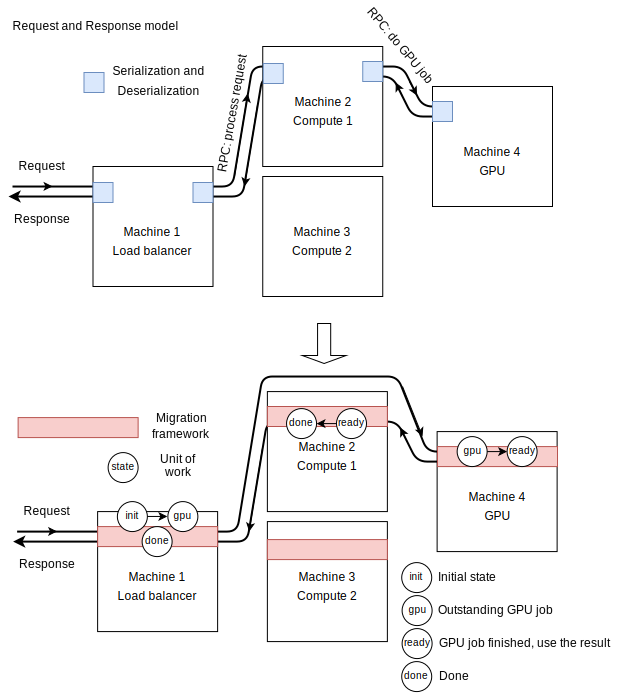
\includegraphics[width=0.8\textwidth]{migration-transport.drawio}
\caption{
    Using a migration platform in state machine based request processing
}
\label{fig:migrationtransport}
\end{figure}

\autoref{fig:migrationtransport} depicts a simple example of this use case.
Each request in this application is an object in the ``init'' state. All of the
data required in the processing of the request is embodied in the object.
To successfully process the request means to transform the object to the
``done'' state and put it on Machine 1 for the result to be committed.
If the object is in the ``gpu'' state, it must be sent to a machine which has access to a
GPU (Machine 4 in this case) for the task to be carried out and the object to be
transformed to the ready state. Each machine does its share of work on the
object, updates the object memory to reflect the update of its state, and
possibly migrates it to another machine based on the new state.

Once again, the application benefits from the reduced overhead of
serialization/deserialization, the ability to balance the load based on the
available resources on the machines, and not having to deal with low level
details of a networking protocol in its core logic.

\subsection{Core properties of a migration framework}
\label{subsec:coreprops}
With the above insights, we can now define migration to stand for
``transferring and object of a particular type to different machine without
serialization/deserialization overheads, through an API that does not
propagate low level networking details to the core application logic''. A
migration framework is the environment that makes this possible. Let us
discuss the properties that such a framework must satisfy.

\paragraph{Real-time performance:}
We define migration delay to be the elapsed time since the start of the
migration of an object until it is successfully migrated to its
destination. Based on the two application types that were discussed,
the most
important feature of a migration framework is its ability to keep the
migration delay small to allow migrations to happen in real-time.
However this is not particularly insightful in designing such a system.
All applications will prefer a smaller end-to-end migration delay
if all of their other metrics are left unchanged.

Similarly exceedingly
    large migration delays will interfere with the performance of
    the applications. Furthermore, directly measuring this
    duration and pursuing its optimization as the main performance goal
    may fail to reflect how the migration process impacts the application.

For example some applications may prioritize responsiveness and
    would trade off
    some of their throughput during the migration process to keep their
    tail latencies low. While there is value in keeping the migration delay
    small, we must
    prioritize maximizing the \emph{usefulness} of the application in
    the distributed setting during the migration, which means we must not only
    minimize the migration delay, but also keep an eye out for preserving
    the application throguhput.

\paragraph{Pluggability and Programmability:}
A fast migration mechanism comes at a cost. After all, each application
could theoretically hand craft and micro-optimize its networking protocol,
but this will complicate the design of the application by propagating
the complexities of the low level protocol into its core.
This will make it difficult to maintain and improve the
application since a small change in how the application does one thing
may break the preconditions of the custom networking protocol.

We therefore aim for zero modifications to the
internals of the applications and minimal additions to the API of their
units of computation. That means if the system designer has already come up
with a way to partition data and computation into units that can run
independently on possibly different machines, the task of integrating the
migration platform into the system to make those units migratable and benfit
from the low overhead transfer and easy load balancing should be trivial.
Similarly the system designer must not worry about breaking the communication
protocol when she makes changes to the internal algorithms in the system.

\section{Computation model and API}
\label{sec:api}
It is not yet clear how a migration platform will be used by the
applications. How do we transfer objects without serializing and deserializing
them? How do we keep the application away low level networking operations while
providing it with a real-time transport? How would the destination application
know what to do with an object that it has just received?

In a simple artificial case where we are migrating a singleton across
the nodes in the cluster some of these issues might sound trivial.
However in more complicated
cases where there can be multiple types of migratable objects in the
system with varying quantities, we need to have a clear picture that
explains what we can do with migratable objects and how the participating
machines play their roles.

In this section we will revisit the two types of applications that
we previously introduced and discuss how they can interface with a
hypothetical migration platform.

\subsection{Listen and serve model}
the first type of application that we discussed can be thought of as a
part of more general family of distributed applications that we call
listen and serve applications. Such systems consist of multiple partitions or
shards, each of which can function on their own. After each shard is
initialized, it will indefinitely execute its ``listen and serve'' routine,
exposing an API through which the other sub-systems of the application
will communicate with that particular shard.

% Since each of these shards operates independently from the other ones and is only
% responsible for a certain part of the workload, the application must also
% provide a routing mechanism to deliver requests to the correct shard.

A randomly sharded distributed
key-value store is an example of this type of applications, where the
partitions of the key-value store naturally map to the partitions in this
model. In the simplest case, each of the partition waits for the incoming
get and set requests, which corresponds to listen and serve in this model.
The application routes the requests to the correct server by keeping track
of which machine is responsible for which set of keys.

\subsection{State machine model}
In this model each task consists of an
independent object in conjunction with the set of operations that must be
executed on the object based on its current state, on a machine that satisfies
certain conditions. Upon receiving the object, a machine will run the
routine that the current state of the object dictates. At the end of the
routine based on the new state of the object the machine may migrate it
elsewhere.

In \autoref{fig:migrationtransport} the routine in the ``gpu''
state could be
``If on a non-GPU machine, migrate to a GPU machine,
while preserving the state, otherwise perform the computation and
go to the ready state''. This
Aside from being able to balance the load of processing the objects through
the cluster, any machine-local resource in the cluster can now be seamlessly
made available to the whole cluster through a migration API.


\subsection{Sending and receiving migratable objects}
\label{subsec:sendrecmig}

A migration platform with any level of programmability and performance
must be usable in a way that can coexist with the application that is
going to use it. To make sure this is the case, we need to specify the
exact set of events that happen towards sending or receiving migratable
objects.

Let us introduce two functions \texttt{send()} and \texttt{receive()} with
the goal of tweaking them until they become suitable for use as the APIs
to the migration platform. \autoref{fig:sendreceive} shows their
declarations in \emph{pseudo-C++}, ignoring parameters such as
source/destination address which are not specific to the migration.

\begin{figure}[t]
\begin{lstlisting}
template<typename T>
void send(T);

template<typename T>
T receive(void);
\end{lstlisting}
\caption{
    Declarations of \texttt{send()} and \texttt{receive()}
}
\label{fig:sendreceive}
\end{figure}

The first point to note about these functions is that they operate on
a typed object, otherwise the caller will need to deal with the complexities
of a low level networking protocol after calling the \texttt{receive()}
function.

Another important and perhaps related point is that \texttt{receive()}
function returns an object, not data. Therefore we have chosen to deal
deal with the object creation ourselves in the framework, without imposing
development or run-time costs of serialization and deserialization on the
system.

How can these too functions be used in conjunction with each other?
In \autoref{subsec:coreprops} we concluded that migrations have to happen in
real-time, but in that case, how can the
sender and receiver rendezvous at the \texttt{send()} and
\texttt{receive()} calls? How do we program the different paths of
execution that might or might not result in the one type of object being
migrated between the two machines?

These are hints that an asynchronous API, particularly with a non-blocking
\texttt{receive()} suits this task much better. However, it is still not clear
how the \texttt{receive()} function will be called and how an execution path
of the core logic finds out about the existence of a received object,
how it distinguishes between the received objects, and how it goes about using
them.

Leaving these issues to be dealt with by the application
fails to address our second goal of programmability and pluggability.
Initializing an object that is migrated from another machine and deciding how
it starts running is a seemingly complex task.
We remedy this issue by taking care of the above tasks as soon as a migrated
object is received. By reducing the degrees of freedom on the destination
machine we can now arrive at a simple, usable API.

\subsection{Migrating runnable objects}
\label{subsec:runnable}
We limit the objects that can be migrated to those
that expose a \texttt{run()} member function to
initialize the object in the destination machine. This will delegate the task
of \emph{using} the object, away from the application and encapsulate it inside
the object itself. To comply with the real-time request of the platform,
the migraiton platform repeatedly calls \texttt{receive()} in parallel to the
application on a separate thread.

To distinguish between different migratable objects of possibly different
types that are present in the system, we declare it the responsibility of the
migration platform to allow the use of multiple
\emph{migration control planes} to be used at the same time by the
application. These control planes must never interfere and act as if they were
operating as the only migration platform in the cluster. They will provide
the send and receive functions in isolation from the one another.
Objects can be initially introduced into the control plane for the
using the control plane's \texttt{accept()} function.

\begin{figure}[tp]
\begin{lstlisting}
class GpuTask {
    State current_state = Init;
    void run() {
        current_node_gpu = GpuDeviceHandle.open();
        ...
        switch(current_state) {
        ...
        case gpu:
            if(!current_node_gpu) {
                // send itself to a machine with a gpu
            }
        }
    }
};

class HashTablePartition {
    void run() {
        router.register(this);
    }
};
\end{lstlisting}
\caption{
    Examples of runnable migratable objects
}
\label{fig:sketchclasses}
\end{figure}

\autoref{fig:sketchclasses} shows a sketch of the migratable objects of
an application which uses migratable control planes to
host both a distributed hash table as a listen and serve type of
application and a state machine based sub-system for running tasks with
heterogeneous resource requirements.

\begin{figure}[tp]
\begin{lstlisting}
int main() {
    GpuTaskControlPlane = MigrationControlPlane<GpuTask>();
    HashTableControlPlane = MigrationControlPlane<HashTablePartition>();

    GpuTaskControlPlane.accept(new GpuTask());

    auto p = new HashTablePartition()
    HashTableControlPlane.accept(p);

    if(machine_id == 1) {
        p.suspend();
        HashTableControlPlane.send(machine_id=1, p);
    }
}
\end{lstlisting}
\caption{
    Example application using runnable migratable objects from \autoref{fig:sketchclasses}
}
\label{fig:sketchmain}
\end{figure}

The \texttt{GpuTask} objects
use a global reference to a GPU device on the machine for their
initialization. Similarly hash table partitions need to register
themselves at the router on the new machine after they are migrated. These
partitions will then start serving their api (e.g. get/set) and wait for
the router to pass to them an incoming get or set request that must be
processed in them.




\autoref{fig:sketchmain} is how we might use the migratable constructs in
\autoref{fig:sketchclasses}. The same program
is run by all of the machines in the cluster. First they create and share
two control planes, one for each migratable type that is used.
Then each applications creates a migratable object of each type and passes
it to the appropriate control plane through its \texttt{accept()} method,
which will call the \texttt{run()} method of the object behind the scenes
for the first time.

As node 1 becomes hypothetically overloaded, it suspends the execution of
    its hash table partition by removing it from the router
    and migrating it to node 2. This will eventually result in the hash table
    control plane of node 1 receiving the migrated partition, calling its
    run() method behind the scenes to register it in the router allowing
    it to be forwarded the appropriate get or set requests from that
    point on.

Every sub-system of the application which needs to be programmed in the
migratable model has to use a separate migration control plane. As an
example, if the application using the types in \autoref{fig:sketchclasses}
were to support a different kind of heterogeneous task programmed in the
state machine model, a third migration control plane must have been created to
be used exclusively for that task.

Details such as how we take away the ownership of the object from the source
machine at the time of the migration will be discussed later.
More importantly, how we can migrate without serialization and deserialization
is also left to be discussed in the next chapter, even though we might
already have an idea about how we can use the type safety in the API of the
migration framework to achieve this.
